\setcounter{figure}{0}

\section{30th April 2023: Triumph Of Righteousness}
\subsection*{Text: Revelation 20:1-15}
  \begin{quote}
  [1] Then I saw an angel coming down from heaven, holding in his hand the key to the bottomless pit and a great chain. [2] And he seized the dragon, that ancient serpent, who is the devil and Satan, and bound him for a thousand years, [3] and threw him into the pit, and shut it and sealed it over him, so that he might not deceive the nations any longer, until the thousand years were ended. After that he must be released for a little while.

  [4] Then I saw thrones, and seated on them were those to whom the authority to judge was committed. Also I saw the souls of those who had been beheaded for the testimony of Jesus and for the word of God, and those who had not worshiped the beast or its image and had not received its mark on their foreheads or their hands. They came to life and reigned with Christ for a thousand years. [5] The rest of the dead did not come to life until the thousand years were ended. This is the first resurrection. [6] Blessed and holy is the one who shares in the first resurrection! Over such the second death has no power, but they will be priests of God and of Christ, and they will reign with him for a thousand years.

  [7] And when the thousand years are ended, Satan will be released from his prison [8] and will come out to deceive the nations that are at the four corners of the earth, Gog and Magog, to gather them for battle; their number is like the sand of the sea. [9] And they marched up over the broad plain of the earth and surrounded the camp of the saints and the beloved city, but fire came down from heaven and consumed them, [10] and the devil who had deceived them was thrown into the lake of fire and sulfur where the beast and the false prophet were, and they will be tormented day and night forever and ever.

  [11] Then I saw a great white throne and him who was seated on it. From his presence earth and sky fled away, and no place was found for them. [12] And I saw the dead, great and small, standing before the throne, and books were opened. Then another book was opened, which is the book of life. And the dead were judged by what was written in the books, according to what they had done. [13] And the sea gave up the dead who were in it, Death and Hades gave up the dead who were in them, and they were judged, each one of them, according to what they had done. [14] Then Death and Hades were thrown into the lake of fire. This is the second death, the lake of fire. [15] And if anyone’s name was not found written in the book of life, he was thrown into the lake of fire.
  \end{quote}
\subsection*{Notes}
\begin{itemize}
  \item{Satan's modus operandi has always been to spread lies to cause people
  to turn away from God and even to turn against God.  We see that starting
  with Adam and Eve.  Last week, we see Jesus (the rider on the white horse)
  triumphing over the beast and the beast's false prophet, symbolising the
  end of His opposition.  Over the last few weeks, we have seen God's wrath
  on His enemies, starting from the fall of Babylon etc.  We should not see
  the multiple accounts of judgment as happening chronologically one after
  another, but we should take all of these accounts as all describing God's
  same judgment, but from different points of view.}
  \item{In our text, the chain that binds Satan and Satan being thrown into
  the pit shows us God's power and sovereignty even over Satan.  Here, the
  reference to $1000$ years is not to be taken literally, but it is to be
  taken metaphorically to mean ``a perfect long time''.  The binding of Satan
  and the $1000$ year duration symbolises the period where Satan is no longer
  able to prevent belief in Jesus.  The $1000$ year period could be the
  period between Christ's first and second coming, so that in this interim
  period, the gospel will effectively be able to convert people to faith in
  Jesus.  And during this period, Satan will not be able to hinder the
  conversion of people to faith in Jesus.  Though Satan can still hinder our
  work, he can't render it totally fruitless.}
  \item{In our text, there is also a contrast between those who shares in the
  first resurrection and those who were raised at the end to be thrown into
  the lake of fire.  Hence we see two types of resurrection; everyone will be
  resurrected in the end (the faithful and the unfaithful), but the faithful
  will be raised to life first to reign together with Christ, and then
  subsequently the unfaithful will be raised to be judged and thrown into the
  lake of fire.  We identify the first group with the faithful because the
  first group is ``those who had been beheaded for the testimony of Jesus,
  $\dots$, and those who had not worshipped the beast of its image and
  $\dots$ (v4)''.}
  \item{In our text again, we also see Satan being released again for a
  little while.  One possible reason for God releasing Satan is for God to
  show that Satan will not repent even after a long time, and also to show
  that the hearts of the unbelievers remain equally hard even after a long
  time.  Here, we see the obstinate rebellion of Man and of Satan.  Here we
  see that without faith in Jesus, Man cannot reform himself to do good even
  in Satan's absence.  We also see that Satan will not reform himself, he
  will continue setting himself in opposition against God.  }
  \item{After Satan's release, he picks up where he left off to continue to
  deceive the nations to gather them for war.  The battle scene here is not
  new, it is similar to the one in chapter $19$.  Hence the outcome is also
  not new, the outcome is the same as was described in chapter 19.  Satan's
  work in stirring up the hardened hearts of Man and to start the war against
  God is described in verses $7-9$, and the result of the war is seen in
  verses $10-15$.  Here we see Satan and the unbelievers being justly judged.}
  \item{The unbelievers here are thrown into the ``lake of fire'' (also known
  as Hell), which is also described as ``darkness'', ``place that the worm
  will not die'', ``place where there is weeping and gnashing of teeth'',
  etc.  There is a lot of very fierce imagery here describing the torment of
  those who died in their unbelief.  We should not take these imagery
  literally, because these images do not describe the full depths of torment
  that the unbelievers feel.}
  \item{For example, Hell is not just a place of physical torment.  Hell is a
  place where the unbelievers are fully and totally cut off from God.  Yet as
  Paul quotes, ``in Him (God) we live and breathe and have our being''.  God
  is our creator and sustainer, and every single person is made for
  fellowship with Him.  Hence for the unbelievers, when this possibility of
  fellowship with God is taken away when they are cast into Hell, the purpose
  that they are made for will never be fulfilled, and the longing in their
  hearts for God that they suppressed in their unbelief will never be
  fulfilled.  As Augustine said, ``our hearts are restless until they rest in
  God'', and for these unbelievers, their hearts will forever remain
  restless.  That itself is the eternal torment that exists in Hell, the
  torment is not physical or emotional but it is on a deeper more
  metaphysical level (it is at the level of the soul).  The physical and
  emotional torment described is just a way for us to scratch the surface of
  the depth of this torment.}
  \item{Yet for us who have faith in Jesus, we can be encouraged that when
  Christ returns, we will share in eternal fellowship with Him and the Father
  through the Holy Spirit.  Our deepest longing to have fellowship with God
  (which we were made for) will be totally and fully fulfilled finally, and
  that is the hope that helps us to be faithful, even unto death.  }
  \item{\begin{figure}[H]
    \centering
    % 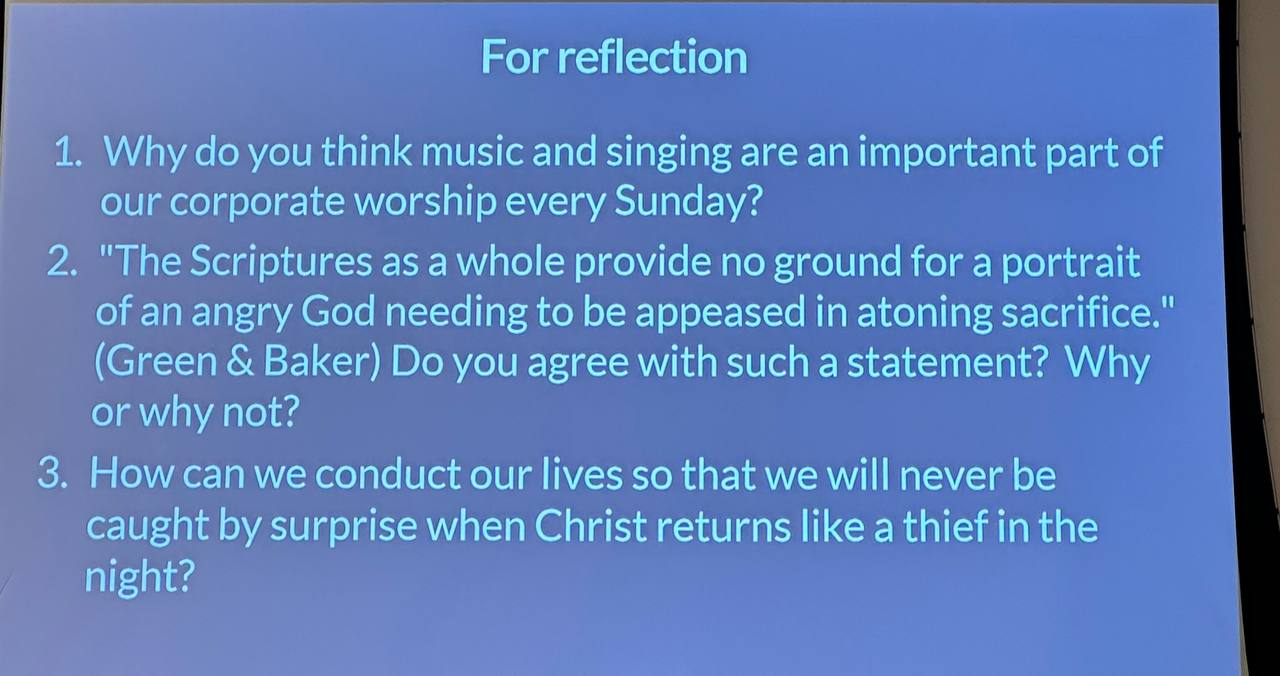
\includegraphics[width=0.8\textwidth, trim={0cm 0cm 0cm 0cm},clip]{Figures/marSermon4Reflections.jpg}
    \includegraphics[width=0.8\textwidth, trim={0cm 0cm 0cm 0cm},clip]{example-image-a}
    \caption[]{Reflection questions for this sermon}
    \label{}
  \end{figure}}
\end{itemize}